\section{Problem Setup}

\subsection{Simplifying Assumptions}

To make the simulation tractable while preserving physical meaning, the following assumptions are adopted throughout:

\begin{itemize}
    \item The gravitational constant is set to $G = 1$. This is a common convention in $N$-body simulations where physical units are scaled so that $G$ drops out of the equations, leaving mass and distance as the only free parameters.
    \item The system is restricted to two dimensions. All position and velocity vectors lie in the $xy$-plane, and no out-of-plane forces are considered.
    \item The star is treated as a fixed gravitational source. Its mass is sufficiently large relative to the planet that its own displacement due to the planet's gravity is negligible. This is the \emph{restricted two-body} or \emph{test-particle} approximation.
    \item The planet's mass cancels out of the equations of motion (as shown in the Formulae section), so only the star's mass enters the dynamics.
\end{itemize}

\subsection{Initial Conditions}

The star is placed at the origin of the coordinate system with mass $M = 1000$ and initial position $\vec{r}_\star = (0,\,0)$. The planet is placed at $\vec{r}_p = (100,\,75)$ and is initially at rest before its orbital velocity is assigned. The initial separation between the two bodies is computed in the \emph{Find Distance} section.

\begin{figure}[H]
\centering
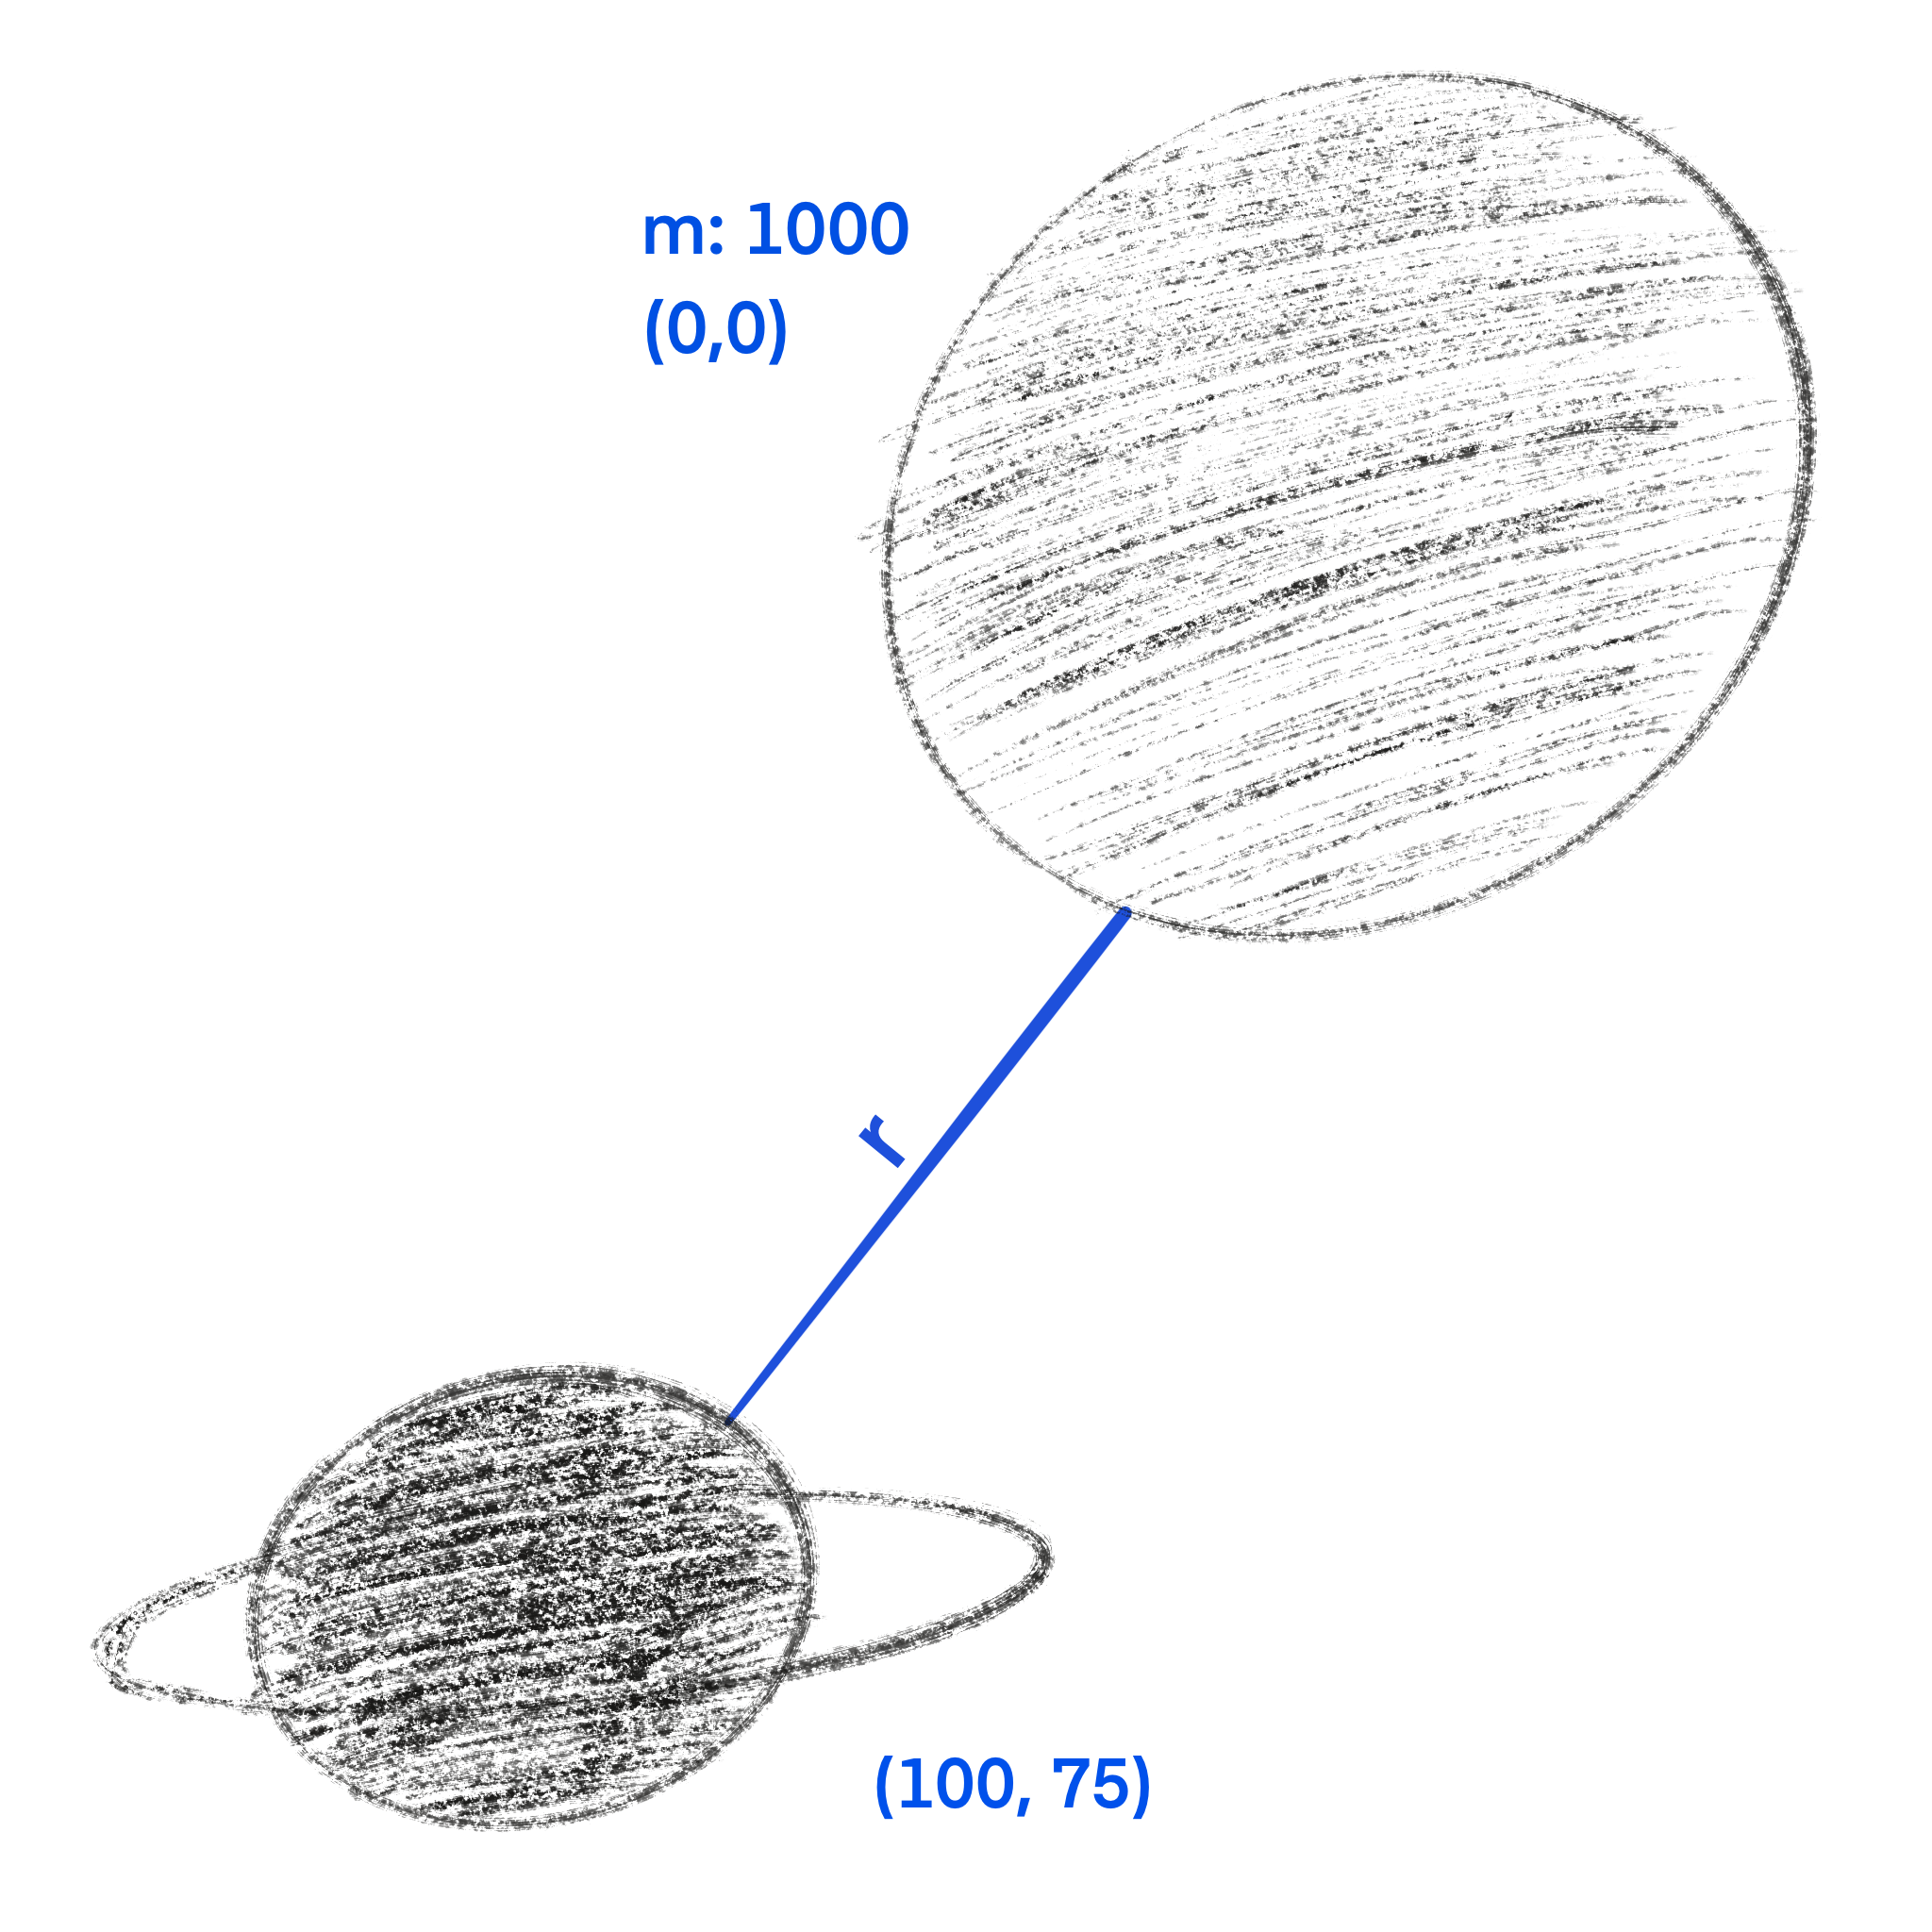
\includegraphics[width=0.8\textwidth]{figures/problem_setup.png}
\caption{Diagram of the initial configuration. The star sits at the origin; the planet is placed at $(100, 75)$.}
\end{figure}

\subsection{Coordinate System}

A standard right-handed Cartesian coordinate system is used, with the positive $x$-axis pointing right and the positive $y$-axis pointing upward. All vector quantities — position, velocity, and acceleration — are stored as two-component vectors, implemented via the \texttt{Vec2} struct in the simulation code.